% ============================================================
% Question Bank: ch05-05 Writing and Solving Inequalities
% Topic Title: Writing and Solving Inequalities
% CCSS: 7.EE.B.4b
% Questions: 27 (15 MC + 6 SA + 6 Graphical)
% ============================================================

% --- Multiple Choice Questions (15) ---

\begin{practiceQuestion}{5-5-q01}{mc}
\begin{questionText}
Solve $3x + 5 > 20$.
\end{questionText}
\choiceA{$x > 5$}
\choiceB{$x > 8\frac{1}{3}$}
\choiceC{$x < 5$}
\choiceD{$x > 25$}
\correctAnswer{A}
\explanation{Subtract $5$: $3x > 15$. Divide by $3$: $x > 5$.}
\end{practiceQuestion}

\begin{practiceQuestion}{5-5-q02}{mc}
\begin{questionText}
Solve $-4n + 12 \leq 0$.
\end{questionText}
\choiceA{$n \leq -3$}
\choiceB{$n \leq 3$}
\choiceC{$n \geq 3$}
\choiceD{$n \geq -3$}
\correctAnswer{C}
\explanation{Subtract $12$: $-4n \leq -12$. Divide by $-4$ and flip the sign: $n \geq 3$.}
\end{practiceQuestion}

\begin{practiceQuestion}{5-5-q03}{mc}
\begin{questionText}
Which inequality represents ``fewer than $20$''?
\end{questionText}
\choiceA{$x \leq 20$}
\choiceB{$x > 20$}
\choiceC{$x < 20$}
\choiceD{$x \geq 20$}
\correctAnswer{C}
\explanation{``Fewer than $20$'' means strictly less than $20$: $x < 20$.}
\end{practiceQuestion}

\begin{practiceQuestion}{5-5-q04}{mc}
\begin{questionText}
Solve $6x - 9 \geq 21$.
\end{questionText}
\choiceA{$x \geq 2$}
\choiceB{$x \geq 5$}
\choiceC{$x \leq 5$}
\choiceD{$x \geq 30$}
\correctAnswer{B}
\explanation{Add $9$: $6x \geq 30$. Divide by $6$: $x \geq 5$.}
\end{practiceQuestion}

\begin{practiceQuestion}{5-5-q05}{mc}
\begin{questionText}
A student solved $-5x + 10 > 30$ and wrote $x > -4$. What error did the student make?
\end{questionText}
\choiceA{Forgot to subtract $10$}
\choiceB{Divided by $5$ instead of $-5$}
\choiceC{Forgot to flip the inequality sign}
\choiceD{Added $10$ instead of subtracting}
\correctAnswer{C}
\explanation{Correct steps: subtract $10$ gives $-5x > 20$. Divide by $-5$ and flip: $x < -4$. The student forgot to flip.}
\end{practiceQuestion}

\begin{practiceQuestion}{5-5-q06}{mc}
\begin{questionText}
Solve $-8x > 24$.
\end{questionText}
\choiceA{$x > -3$}
\choiceB{$x < -3$}
\choiceC{$x > 3$}
\choiceD{$x < 3$}
\correctAnswer{B}
\explanation{Divide by $-8$ and flip the sign: $x < -3$.}
\end{practiceQuestion}

\begin{practiceQuestion}{5-5-q07}{mc}
\begin{questionText}
You have $\$85$ and spend $\$12$ per day. You want to keep at least $\$25$. Which inequality finds the number of days $d$ you can spend?
\end{questionText}
\choiceA{$85 + 12d \geq 25$}
\choiceB{$85 - 12d \leq 25$}
\choiceC{$85 - 12d \geq 25$}
\choiceD{$12d - 85 \geq 25$}
\correctAnswer{C}
\explanation{Start with $\$85$, subtract $\$12$ per day, need at least $\$25$ remaining: $85 - 12d \geq 25$.}
\end{practiceQuestion}

\begin{practiceQuestion}{5-5-q08}{mc}
\begin{questionText}
Solve $\dfrac{x}{5} + 3 < 7$.
\end{questionText}
\choiceA{$x < 50$}
\choiceB{$x < 2$}
\choiceC{$x < 20$}
\choiceD{$x < 4$}
\correctAnswer{C}
\explanation{Subtract $3$: $\frac{x}{5} < 4$. Multiply by $5$: $x < 20$.}
\end{practiceQuestion}

\begin{practiceQuestion}{5-5-q09}{mc}
\begin{questionText}
Which value of $x$ is NOT a solution to $5x - 2 > 13$?
\end{questionText}
\choiceA{$x = 4$}
\choiceB{$x = 5$}
\choiceC{$x = 10$}
\choiceD{$x = 3$}
\correctAnswer{D}
\explanation{Solve: $5x > 15$, so $x > 3$. $x = 3$ does not satisfy $x > 3$ (strict inequality). Check: $5(3) - 2 = 13$, not greater than $13$.}
\end{practiceQuestion}

\begin{practiceQuestion}{5-5-q10}{mc}
\begin{questionText}
Solve $4x + 8 \leq 32$.
\end{questionText}
\choiceA{$x \leq 10$}
\choiceB{$x \leq 6$}
\choiceC{$x \geq 6$}
\choiceD{$x \leq 40$}
\correctAnswer{B}
\explanation{Subtract $8$: $4x \leq 24$. Divide by $4$: $x \leq 6$.}
\end{practiceQuestion}

\begin{practiceQuestion}{5-5-q11}{mc}
\begin{questionText}
A band needs to raise more than $\$300$ for new uniforms. They charge $\$7$ per car wash and already have $\$65$. Which inequality finds the number of car washes $c$ they need?
\end{questionText}
\choiceA{$7c + 65 \leq 300$}
\choiceB{$7c - 65 > 300$}
\choiceC{$7c + 65 > 300$}
\choiceD{$65c + 7 > 300$}
\correctAnswer{C}
\explanation{Car wash income is $7c$. Add $\$65$ already raised: $7c + 65 > 300$.}
\end{practiceQuestion}

\begin{practiceQuestion}{5-5-q12}{mc}
\begin{questionText}
Solve $-7x - 5 \geq 16$.
\end{questionText}
\choiceA{$x \geq -3$}
\choiceB{$x \leq -3$}
\choiceC{$x \geq 3$}
\choiceD{$x \leq 3$}
\correctAnswer{B}
\explanation{Add $5$: $-7x \geq 21$. Divide by $-7$ and flip: $x \leq -3$.}
\end{practiceQuestion}

\begin{practiceQuestion}{5-5-q13}{mc}
\begin{questionText}
Which inequality means ``at least $40$''?
\end{questionText}
\choiceA{$x > 40$}
\choiceB{$x < 40$}
\choiceC{$x \leq 40$}
\choiceD{$x \geq 40$}
\correctAnswer{D}
\explanation{``At least $40$'' means $40$ or more: $x \geq 40$.}
\end{practiceQuestion}

\begin{practiceQuestion}{5-5-q14}{mc}
\begin{questionText}
Solve $9 - 3x < -6$.
\end{questionText}
\choiceA{$x < 5$}
\choiceB{$x > 5$}
\choiceC{$x < -5$}
\choiceD{$x > -5$}
\correctAnswer{B}
\explanation{Subtract $9$: $-3x < -15$. Divide by $-3$ and flip: $x > 5$.}
\end{practiceQuestion}

\begin{practiceQuestion}{5-5-q15}{mc}
\begin{questionText}
A student must score at least $90$ points on a test. Each question is worth $6$ points and there are $5$ bonus points. Which inequality finds the minimum questions $q$ answered correctly?
\end{questionText}
\choiceA{$6q + 5 > 90$}
\choiceB{$6q - 5 \geq 90$}
\choiceC{$6q + 5 \geq 90$}
\choiceD{$5q + 6 \geq 90$}
\correctAnswer{C}
\explanation{Score $= 6q + 5$, needs at least $90$: $6q + 5 \geq 90$.}
\end{practiceQuestion}

% --- Short Answer Questions (6) ---

\begin{practiceQuestion}{5-5-q16}{sa}
\begin{questionText}
Solve $5x + 12 > 42$.
\end{questionText}
\correctAnswer{$x > 6$}
\explanation{Subtract $12$: $5x > 30$. Divide by $5$: $x > 6$.}
\end{practiceQuestion}

\begin{practiceQuestion}{5-5-q17}{sa}
\begin{questionText}
Solve $-6n + 18 \leq -12$.
\end{questionText}
\correctAnswer{$n \geq 5$}
\explanation{Subtract $18$: $-6n \leq -30$. Divide by $-6$ and flip: $n \geq 5$.}
\end{practiceQuestion}

\begin{practiceQuestion}{5-5-q18}{sa}
\begin{questionText}
Write and solve an inequality: ``A number $x$ multiplied by $3$, then decreased by $4$, is at most $11$.''
\end{questionText}
\correctAnswer{$3x - 4 \leq 11$; $x \leq 5$}
\explanation{$3x - 4 \leq 11$. Add $4$: $3x \leq 15$. Divide by $3$: $x \leq 5$.}
\end{practiceQuestion}

\begin{practiceQuestion}{5-5-q19}{sa}
\begin{questionText}
Solve $10 - 4x \geq 26$.
\end{questionText}
\correctAnswer{$x \leq -4$}
\explanation{Subtract $10$: $-4x \geq 16$. Divide by $-4$ and flip: $x \leq -4$.}
\end{practiceQuestion}

\begin{practiceQuestion}{5-5-q20}{sa}
\begin{questionText}
A family wants to save more than $\$200$ for a trip. They save $\$15$ per week and have already saved $\$50$. Write and solve an inequality for the number of weeks $w$.
\end{questionText}
\correctAnswer{$15w + 50 > 200$; $w > 10$}
\explanation{$15w + 50 > 200$. Subtract $50$: $15w > 150$. Divide by $15$: $w > 10$. They need more than $10$ weeks.}
\end{practiceQuestion}

\begin{practiceQuestion}{5-5-q21}{sa}
\begin{questionText}
Solve $\dfrac{x}{3} - 5 \leq 1$.
\end{questionText}
\correctAnswer{$x \leq 18$}
\explanation{Add $5$: $\frac{x}{3} \leq 6$. Multiply by $3$: $x \leq 18$.}
\end{practiceQuestion}

% --- Graphical MC Questions (3) ---

\begin{practiceQuestion}{5-5-q22}{gmc}
\begin{questionText}
Which inequality is represented by the number line below?

\begin{center}
\begin{tikzpicture}[scale=0.7]
  \draw[thick,->] (-1,0) -- (10,0);
  \foreach \x in {0,...,9} \draw (\x,0.15) -- (\x,-0.15) node[below] {$\x$};
  \draw[thick,funBlue,->] (3,0) -- (10,0);
  \fill[funBlue] (3,0) circle (4pt);
\end{tikzpicture}
\end{center}
\end{questionText}
\choiceA{$x > 3$}
\choiceB{$x \geq 3$}
\choiceC{$x < 3$}
\choiceD{$x \leq 3$}
\correctAnswer{B}
\explanation{The closed circle at $3$ means $3$ is included, and shading to the right means values greater than or equal to $3$: $x \geq 3$.}
\end{practiceQuestion}

\begin{practiceQuestion}{5-5-q23}{gmc}
\begin{questionText}
Which inequality is represented by the number line below?

\begin{center}
\begin{tikzpicture}[scale=0.7]
  \draw[thick,->] (-6,0) -- (4,0);
  \foreach \x in {-5,...,3} \draw (\x,0.15) -- (\x,-0.15) node[below] {$\x$};
  \draw[thick,funBlue,<-] (-6,0) -- (-2,0);
  \draw[thick,funBlue,fill=white] (-2,0) circle (4pt);
\end{tikzpicture}
\end{center}
\end{questionText}
\choiceA{$x \leq -2$}
\choiceB{$x > -2$}
\choiceC{$x < -2$}
\choiceD{$x \geq -2$}
\correctAnswer{C}
\explanation{The open circle at $-2$ means $-2$ is not included, and shading to the left means values less than $-2$: $x < -2$.}
\end{practiceQuestion}

\begin{practiceQuestion}{5-5-q24}{gmc}
\begin{questionText}
A balance scale shows the left side weighing more. Which inequality represents this?

\begin{center}
\begin{tikzpicture}[scale=0.7]
  % Fulcrum
  \draw[thick] (0,-0.5) -- (-0.4,-1.2) -- (0.4,-1.2) -- cycle;
  % Beam (tilted left side down)
  \draw[thick] (-4,-0.3) -- (4,0.3);
  % Left pan (lower)
  \draw[thick] (-4,-0.3) -- (-4.5,-0.8) -- (-3.5,-0.8) -- (-4,-0.3);
  \draw[thick,fill=funBlue!20] (-4.5,-0.8) -- (-4.5,-1.1) -- (-3.5,-1.1) -- (-3.5,-0.8) -- cycle;
  \node at (-4,-0.95) {\small $2x + 9$};
  % Right pan (higher)
  \draw[thick] (4,0.3) -- (4.5,-0.2) -- (3.5,-0.2) -- (4,0.3);
  \draw[thick,fill=funOrange!20] (4.5,-0.2) -- (4.5,-0.5) -- (3.5,-0.5) -- (3.5,-0.2) -- cycle;
  \node at (4,-0.35) {\small $15$};
\end{tikzpicture}
\end{center}
\end{questionText}
\choiceA{$2x + 9 < 15$}
\choiceB{$2x + 9 = 15$}
\choiceC{$2x + 9 > 15$}
\choiceD{$2x + 9 \leq 15$}
\correctAnswer{C}
\explanation{The left side is heavier (tilted down), so $2x + 9 > 15$.}
\end{practiceQuestion}

% --- Graphical SA Questions (3) ---

\begin{practiceQuestion}{5-5-q25}{gsa}
\begin{questionText}
Write the inequality shown on the number line below.

\begin{center}
\begin{tikzpicture}[scale=0.7]
  \draw[thick,->] (-2,0) -- (8,0);
  \foreach \x in {-1,...,7} \draw (\x,0.15) -- (\x,-0.15) node[below] {$\x$};
  \draw[thick,funBlue,<-] (-2,0) -- (4,0);
  \fill[funBlue] (4,0) circle (4pt);
\end{tikzpicture}
\end{center}
\end{questionText}
\correctAnswer{$x \leq 4$}
\explanation{The closed circle at $4$ means $4$ is included. Shading to the left means all values less than or equal to $4$: $x \leq 4$.}
\end{practiceQuestion}

\begin{practiceQuestion}{5-5-q26}{gsa}
\begin{questionText}
Solve $-2x + 6 > 14$ and describe the graph on a number line.

\begin{center}
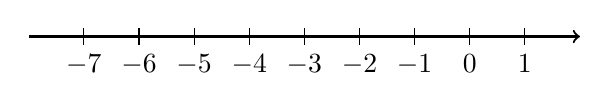
\begin{tikzpicture}[scale=0.7]
  \draw[thick,->] (-8,0) -- (2,0);
  \foreach \x in {-7,...,1} \draw (\x,0.15) -- (\x,-0.15) node[below] {$\x$};
\end{tikzpicture}
\end{center}
\end{questionText}
\correctAnswer{$x < -4$; open circle at $-4$, shade left}
\explanation{Subtract $6$: $-2x > 8$. Divide by $-2$ and flip: $x < -4$. Open circle at $-4$, shade left.}
\end{practiceQuestion}

\begin{practiceQuestion}{5-5-q27}{gsa}
\begin{questionText}
Write the inequality shown on the number line below and give one integer solution.

\begin{center}
\begin{tikzpicture}[scale=0.7]
  \draw[thick,->] (-1,0) -- (12,0);
  \foreach \x in {0,...,11} \draw (\x,0.15) -- (\x,-0.15) node[below] {$\x$};
  \draw[thick,funBlue,->] (7,0) -- (12,0);
  \draw[thick,funBlue,fill=white] (7,0) circle (4pt);
\end{tikzpicture}
\end{center}
\end{questionText}
\correctAnswer{$x > 7$; one solution is $x = 8$}
\explanation{The open circle at $7$ means $7$ is not included. Shading to the right means $x > 7$. One integer solution is $8$.}
\end{practiceQuestion}
